%!TEX root = ../bare_adv.tex
\subsection{Maximum Speed}
\label{sec:speed}
We now explain what is meant by the maximum speed of an object.
When an object is outside the range of any sensors it is said to be vacant.
When an object is in a vacant time interval its position can be narrowed down to the cell it is located in, see Figure \ref{fig:vacant}. 
Further its position can be narrowed down based on the maximum speed of the object and the time interval between leaving the range of the sensor and now, formally $A_{speed} V_{max}\cdot\Delta t_1$. 
The speed of an object type may vary, e.g. a human have a maximum recorded speed of 37.58 km/h~\cite{bolt}.
We view the range of the sensor $P_1$ as a circle with the sensors maximum range as radius, we denote this $R_1$, see Figure \ref{fig:speed1}.
Knowing the maximum speed of the object a circle can be drawn from the point where the object left the vicinity of the sensor, see $R_4$.
It is often not know at which point the object left the range of the sensor, but only when it left.
Regardless of which point the object left the vicinity an maximum travelled range can be calculated. 
By drawing a circle with the radius $R_5$ ($R_1 + R_4$) the maximum area which the object can have moved is found.  
The next reading from a new sensor of the object can be used to create an oval between the two sensor readings, see Figure \ref{fig:speed2}.  
The oval is bounded by the maximum speed of the object and the time between the two readings. 
\begin{figure}%
\centering
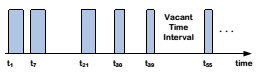
\includegraphics[width=\columnwidth]{images/vacant.png}%
\caption{The x-axis show the timestamps where the object enters the vicinity of a sensor. The colored areas are the time interval where the object in within the range of the sensor. The figure is take from~\cite{Jensen:2009:GMB:1590953.1591000}.}%
\label{fig:vacant}%
\end{figure}
\begin{figure}%
\centering
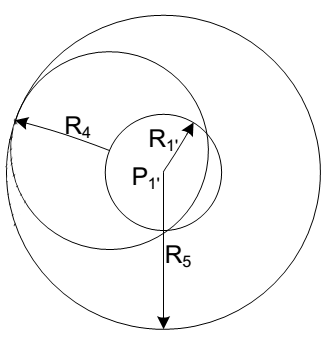
\includegraphics[width=0.5\columnwidth]{images/speed.png}%
\caption{The area that the object can move with in $V_{max}\cdot\Delta t_1$. The red area is the intersection of the cell and $A_{speed}$. The figure is adapted from~\cite{Jensen:2009:GMB:1590953.1591000}.}%
\label{fig:speed1}%
\end{figure}
\begin{figure}%
\centering
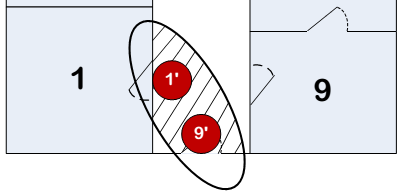
\includegraphics[width=0.8\columnwidth]{images/speed2.png}%
\caption{This figure illustrates the area where the object can be located in the vacant time between the two sensor reading. The figure is take from~\cite{Jensen:2009:GMB:1590953.1591000}.}%
\label{fig:speed2}%
\end{figure}
We can further improve the area in which the object can be in by taking advantage of the building layout, by assuming the object cannot pass through walls. 




